\documentclass[11pt,a4paper]{report}
\usepackage[latin1]{inputenc} 	%encodage caract

\usepackage[T1]{fontenc}
\usepackage{fourier}
\usepackage{txfonts}

\usepackage{textcomp}		%caract�res sp�ciaux
\usepackage{color}			%texte en couleur
\usepackage{graphicx}		%pour les figures
\pagestyle{empty}			%pas d'en-t�te ni pieds-de-pages
\usepackage{fullpage}		%toute la largeur

\usepackage[backend=bibtex,sorting=ydnt,bibstyle=alphabetic,url=false,doi=false]{biblatex}
\addbibresource{Doc.bib}

%% HyperLinks %%
\usepackage{hyperref}	% interactive links
% options and commands for clickable urls and emails
\hypersetup{colorlinks=true,linkcolor=black,urlcolor=blue}

\usepackage{fancybox}
\usepackage[verbose]{wrapfig}	%wrap figure with text
\usepackage{subfig}

\usepackage[nobottomtitles*]{titlesec}

%% Evite totalement les veuves et orphelines
\widowpenalty=10000
\clubpenalty=10000

\usepackage{microtype}

\begin{document}

\begin{titlepage}
\centering
\fontsize{100}{120} \selectfont \textls[250]{OMax}\\
\smallskip
\Huge \textls[150]{\textit{The Software Improviser}}\\
\smallskip
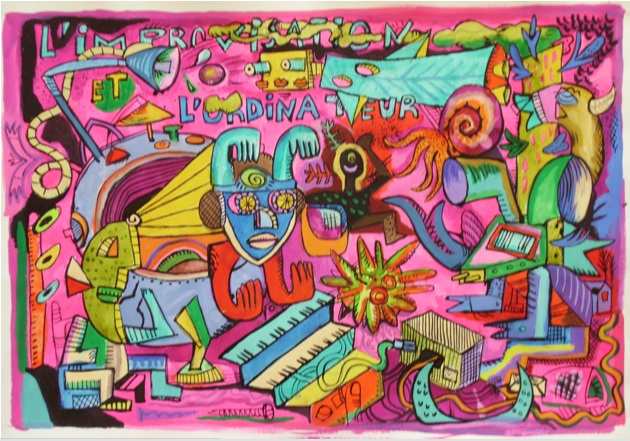
\includegraphics[scale=.52]{AfficheMartin.jpg}\\
\hspace{10em} \scriptsize \textcopyright \textit{Marin Lartigues}\\
\vspace{10em}
\Huge Version 4.5.x\\
\vfill
\normalsize
OMax design and development by G.~Assayag, G.~�Bloch, M.~Chemillier, B. Levy with S.~Dubnov\\
Documentation by B.~Levy\\
\bigskip
\raggedleft \textcopyright \  IRCAM, 2004-2012
\end{titlepage}

\newpage
\thispagestyle{empty}
\mbox{}

\tableofcontents
\setcounter{page}{1}
%\listoffigures

%%%%%%%%%%%%%%%%%%%%%%
\chapter{Introduction}
\section{System Requirements}
\subsubsection{Hardware}
OMax 4.5.3 has been developed and tested for Apple computers based on an Intel processor only. It has been extensively used on laptops of the Macbook Pro series, models going from Macbook Pro 3,2 (2007 with Core 2 Duo processor) to the most recent Unibody models.
\subsubsection{Software}
OMax 4.5.3 has been developed and used in Max/MSP 5 in its most recent (and last) version, 5.1.9. It has been tested on Max 6.0.8 and positive feedback has been given on tests on Max 6.1.x as well.\\
%OMax 4.5.1 uses also third party externals for Max/MSP 5 as \textsf{yin\textasciitilde} and \textsf{supervp.scrub\textasciitilde} developed at IRCAM and distributed through its software portal \href{http://forumnet.ircam.fr/}{\textit{Forumnet}} and \textsf{zsa.mfcc\textasciitilde} and \textsf{zsa.dist} which are part of the \textit{zsa.descriptors} package developed by E. Jourdan and downloadable on his website \href{http://www.e--j.com/}{\textit{e--j}}.

%%
\section{OMax Principles}\label{principles}
\subsection{Fundamentals}
OMax is an improvising software which uses on-the-fly learning and generating from a live source. It is capable of simultaneously \textit{listening} to the audio stream of a musician, \textit{extracting} information from that stream, \textit{modeling} this information into a complex formal structure (think of a musical roadmap), then \textit{navigating} this structure by recombining the musical material to create variation(s) or ``clone(s)'' of the input. OMax has no \textit{a priori} knowledge or rules to guess or infer any specific analysis of the input based on a particular music theory (it is said \textit{agnostic}). Thus its versatility and adaptability. OMax can either input and generate MIDI information or input and output an audio signal, in which case it uses a recording of the very musician's sound, thus enforcing the ``cloning'' effect.
\subsection{Style Modelling}
``\textit{By Style Modelling, we imply building a computational representation of the musical surface that captures important stylistic features hidden in the way patterns of rhythm, melody, harmony and polyphonic relationships are interleaved and recombined in a redundant fashion.}''% \ref{}
. In other words, style modeling is the extraction of implicit rules from a musical material (often referred as the source). Whether the system infers the implicit rules of the source or mimics the surface without trying to guess these rules depends on the representation model used.\\
In this field, investigations have been done (in collaboration with Shlomo Dubnov) with dictionary based models such as LZ compression algorithm (Incremental Parsing (IP) methods) or Prediction Suffix Trees% as reviewed in \ref{}
. Both methods build a tree encoding patterns occurrences and allows to calculate probabilities on the continuation of a given pattern.% A rather large review of music generation methods is given \ref{}.
\\
In the years 2001-2002 %\ref{} 
the Music Representation team in IRCAM started to use a novel representation of pattern repetition, Factor Oracle, coming from the genetic research on patterns in genome. Since then, they studied and successfully used this representation for style modelling and music generation and built OMax, a real-time improvising system using stylistic reinjection.
\subsection{Stylistic Reinjection}
The musical hypothesis behind stylistic reinjection is that an improvising performer is informed continually by several sources, some of them involved in a complex feedback loop. The performer listens to his partners. He also listens to himself while he is playing, and the instantaneous judgment he bears upon what he is doing interferes with the initial planning in a way that could change the plan itself and open up new directions.\\
Sound images of his present performance and of those by other performers are memorized and drift back in memory from present to the past. From the long-term memory they also act as inspiring sources of material that would eventually be recombined to form new improvised patterns. Musical patterns are supposed not to be stored in memory as literal chains, but rather as compressed models, that may develop into similar but not identical sequences: this is one of the major issues behind the balance of recurrence and innovation that makes an interesting improvisation.\\
The idea of stylistic reinjection is to reify, using the computer as an external memory, this process of reinjecting musical figures from the past in a recombined fashion, providing an always similar but always innovative reconstruction of the past. To that extent, OMax, as a virtual partner will look familiar, as well as challenging, to his human partner. The interesting thing is to see how the human partner reacts to his ``clone'' and changes his improvisation accordingly.

\newpage

%%
\section{Quick Start}\label{quick}
\subsection{Audio}
\begin{enumerate}
	\item Starting point to get OMax working (after checking the system requirements) is to \textbf{load the \textsf{OMax.4.5.x.maxpat} patch in Max 5}. This patch is highlighted in red in the \textsf{OMax Patches\&Objects} folder. Or you can use the alias pointing to it present in the \textsf{OMax4.5.x} folder. It may take one or two minutes as the patch embeds a lot of others. It should print about 35 lines in your Max window with the credits for external objects and \textsf{OMax.data}, \textsf{OMax.oracle} and \textsf{OMax.buffers} declarations. However, none of them should be red (error message). Next steps will make reference to the capture presented Figure~\ref{quickaudio}.
	\item If you want to use OMax on a live input, \textbf{adjust the channels} (accordingly to your hardware and Max I/O mappings) then \textbf{check the \textsf{Input} toggle} (frames 2, top left corner of the patch).\\
NB: The first channel (named \textsf{rec}) is used to record the sound in a buffer (and replayed later on) while the second channel (named \textsf{dtct}) is fed into the detection (analysis) system. These two channel can receive the same stream if you use only one microphone.\\
If you want to use OMax on a sound file, click on the \textsf{open} message of the \textsf{Play file} box and choose an aiff file in the navigator popping up. Checking and unchecking the toggle (frame 2b, top left corner of the box) will start and stop the playing of your file once the audio is turned on.
	\item Provided that you had no errors in the Max window when you loaded the patch, you can now \textbf{turn on the audio} with the ``speaker'' button (frame 3, bottom right side of the patch).
	\item You can \textbf{check and adjust the level} of the sound arriving to OMax with the horizontal vumeters (and their overlaid sliders) in and on the right of the \textsf{Record} box (frame 4). You can also \textbf{monitor} this stream by checking the top left toggle of the \textsf{Monitor} box (frame 4b) ---~you may need to adjust the channels of your monitoring system with the numbers in the same box.\\
The \textsf{Pitch} and \textsf{Spectral} boxes \textbf{LEDs should start flashing} (frame 4) as the sound gets through. It indicates that they are detecting some activity and able to extract information from the audio. Otherwise you need to continue adjusting levels and/or detection parameters (see~\ref{pitchsection} or \ref{spectralsection}).
	\item When you are ready, you can \textbf{start recording and learning} by checking the big toggle labelled \textsf{Start Learning} on the top of the patch (frame 5).\\
If you work with a sound file, you can stop and start reading the file again from the beginning with the toggle of the \textsf{Play file} box (frame 2b).\\
Model should start being built, \textsf{Size} and \textsf{Hi Ctxt} of the \textsf{Dual\textunderscore MIDI} and \textsf{Dual\textunderscore SP} boxes should start growing.
	\item You can \textbf{activate the visualization} of the knowledge by checking the top toggle of the \textsf{Visu} box (frame 6) and looking in the Jitter window. At least an horizontal black line should appear and hopefully some white and grey arcs below and above this timeline proving that OMax is recognizing some interesting patterns.
	\item OMax is now ready to improvise! \textbf{Check} the top left toggle of \textbf{one of the players and it should start playing} (frames 7). You can adjust the channel and volume of each of the players in the \textsf{Output} box right below.
	\item Hit the \textsf{Stop!} button (frame 8, on the top of the patch) to \textbf{stop all the players at once}. And \textbf{reset} the Audio part of OMax \textbf{with the \textsf{Reset} button} underneath the \textsf{Start Learning} toggle (frame 8, on the top of the patch) and to be ready to start again a new improvisation.
\end{enumerate}
\begin{figure}[h]
	\centering
	\centerline{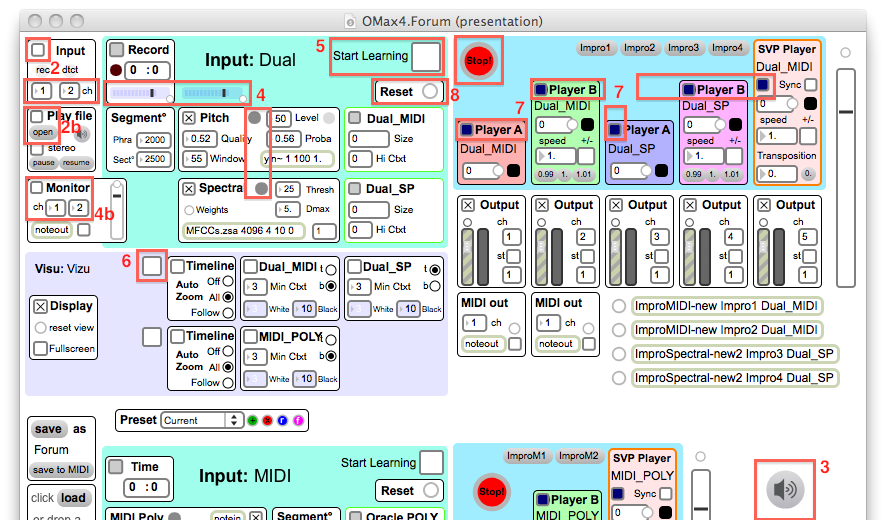
\includegraphics[width=1.2\linewidth]{QuickStart-Audio.png}}
	\caption{Audio Quick Start}
	\label{quickaudio}
\end{figure}

\clearpage
\subsection{MIDI}
\begin{enumerate}
	\item Starting point to get OMax working (after checking the system requirements) is to \textbf{load the \textsf{OMax.Forum} patch in Max 5}. This patch is highlighted in red in the \textsf{OMax4.5} folder. It may take one or two minutes as the patch embeds a lot of others. It should print about 35 lines in your Max window with the credits for external objects and \textsf{OMax.data}, \textsf{OMax.oracle} and \textsf{OMax.buffers} declarations. However, none of them should be red (error message). Next steps will make reference to the capture presented Figure~\ref{quickmidi}.
	\item First you need to \textbf{define a MIDI input} to receive data from by double-click on the \textsf{notein} object in the \textsf{MIDI Poly} box (frame 2). You can also adjust the channel you want to listen to with the number box right below (frame 2). A value of $-1$ means \textit{all channels}.\\
NB: if you want to play a MIDI file and feed it to OMax, you need to use an external software as \href{http://www.ronimusic.com/}{\textit{Sweet MIDI Player}} to play and route the MIDI stream to Max/MSP.\\
The \textbf{LED} of the \textsf{MIDI Poly} box should start flashing as soon as you receive MIDI data.
	\item You are now set to \textbf{start the learning} of OMax by checking the toggle labelled \textsf{Start Learning} (frame 3, on the top of the MIDI part of the patch).
	\item You can \textbf{activate the visualization} of the knowledge by checking the bottom toggle of the \textsf{Visu} box (frame 4) and looking in the Jitter window. At least an horizontal black line should appear and hopefully some white and grey arcs below and above this timeline proving that OMax is recognizing some interesting patterns.
	\item Before making OMax improvise, you need to \textbf{adjust the MIDI output of the players}. Double-click on the \textsf{noteout} box of each of them (frame 5) to decide if you want to use the default synthesizer of the Apple Operating System, \textit{AU DLS Synth} or if you want to send the MIDI stream to another synthesizer you may have on your computer.
	\item OMax is now ready to improvise! \textbf{Check} the top left toggle of \textbf{one of the players and it should start playing} (frames 6).
	\item Hit the \textsf{Stop!} button (frame 7, near the players) to \textbf{stop all the players at once}. And \textbf{reset} the MIDI part of OMax \textbf{with the \textsf{Reset} button} on the left of the \textsf{Stop!} button (frame 7) to be ready to start again a new improvisation.
\end{enumerate}
\begin{figure}[h]
	\centering
	\centerline{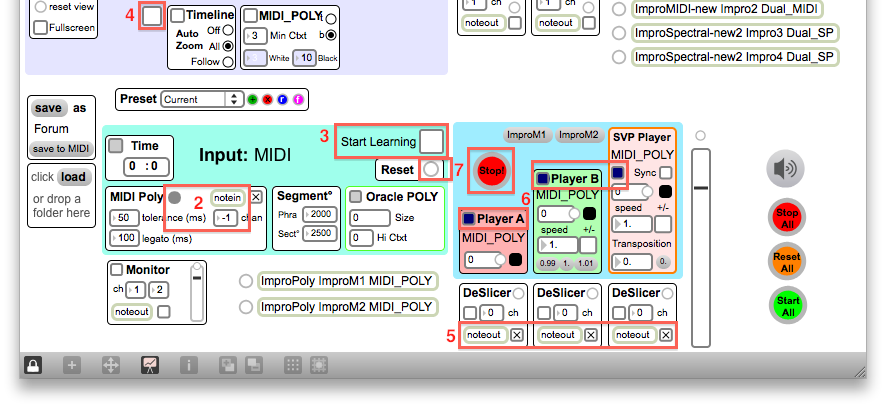
\includegraphics[width=1.2\linewidth]{QuickStart-MIDI.png}}
	\caption{MIDI Quick Start}
	\label{quickmidi}
\end{figure}

\clearpage
%%
\section{Architecture}
\subsection{Overall view}\label{overview}
From a very distant point of view, OMax is built in two parts. A first ensemble is in charge of the listening and learning process and a second ensemble is the improvising part itself.
%To achieve the improvising part of OMax, it is necessary however that learning part construct properly the Factor Oracle model previously mentioned.
The analysis is conceptually divided in three stages. A first stage extracts from the incoming stream some abstract description based on signal processing principles (which will be described later in this documentation). Once this \textbf{detection} has been done, a \textbf{segmentation} stage takes the abstract stream (of numbers mostly) from the detection to aggregate them into consistent units that have a symbolic coherence and a defined value.\\
For example, in the common case of pitch information, the detection stage will be an algorithm for fundamental frequency extraction. It will output a continuous stream of frequencies that need to be filtered and grouped by the segmentation to give a symbolic information of note defined by its onset, offset and pitch value (possibly given also with a velocity value).\\
The result of these two steps of analysis is a symbolic representation of the input stream that can be learnt in the pattern recognition model of OMax. This \textbf{modelling} is done by constructing the Factor Oracle graph previously mentioned.
\begin{figure}[h]
	\centering
	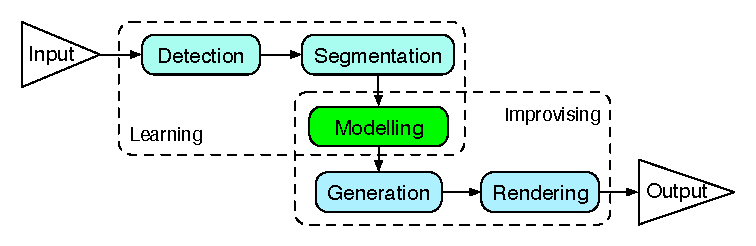
\includegraphics{Overall.eps}
	\caption{Overall architecture of OMax}
	\label{overall}
\end{figure}
\par
Once the building of the model has started, the improvising part of OMax is able to navigate in this model to create a virtual improviser (often referred as a ``clone'') which plays variations on the learnt sequence. A first block reads the model and generates a path for an improvisation. This \textbf{generation} block sends (usually along the navigation) the informations about this path to the \textbf{rendering} block which is in charge of retrieving the effective recorded elements (typically the audio chunks) to read and produce the sound of the ``clone''.

%
\subsection{Functions\label{funct}}
In a more detailed view of OMax, we can describe the different parts previously presented with more blocks.
\begin{figure}[h]
	\centering
	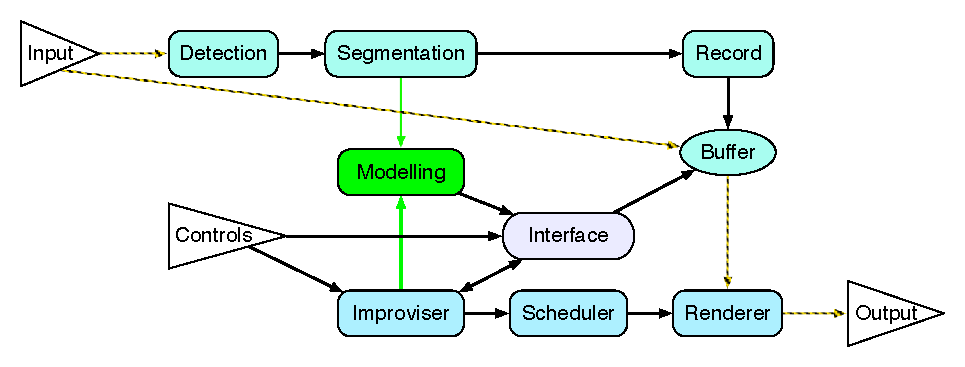
\includegraphics{Functions.eps}
	\caption{Functions in OMax}
	\label{functions}
\end{figure}
As suggested, there is naturally a recording part in the learning ensemble of OMax composed of a \textbf{buffer} and a \textbf{record} agent. The rendering part of the improvising ensemble can also be divided in two different elements : the \textbf{scheduler} is in charged of putting the path (in the learnt knowledge) \textit{in time} then the \textbf{renderer} read the recorded buffer to get the information to output the actual sound material.
\par
The visualisation part is one of the main novelty in OMax 4.x (compared to the previous versions). It allows the user to see in real-time on the \textbf{interface} the current state of the model and interact with the improvising part, with regards to this state.

%
\subsection{Externals}
The second main novelty in OMax 4.x is the integration of OMax in the Max/MSP environment solely. On the diagram~\ref{functions}, with respect to Max/MSP conventions, black links represent message connection while yellow and black arrows are audio connections. The green links show the connections with the knowledge model which required specific external objects for Max/MSP developed in C/C++ especially for OMax.
\begin{figure}[h]
	\centering
	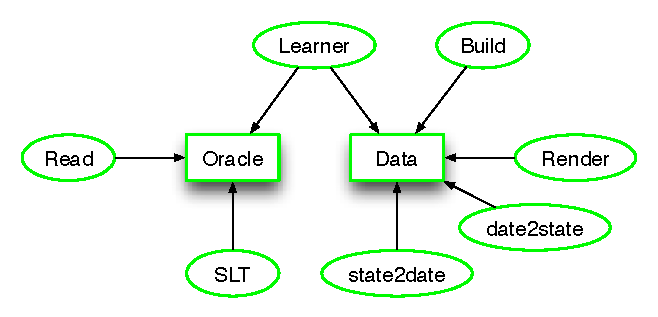
\includegraphics{Externals.eps}
	\caption{External objects for OMax 4.x}
	\label{externals}
\end{figure}
A collection of 9 external objects for Max/MSP is provided with OMax. They are all named with the prefix \textit{OMax.} They implement two data structures: one (\textbf{OMax.oracle}) is the Factor Oracle graph structure, the other one (\textbf{OMax.data}) holds the musical (symbolic) content of the input sequence. The other objects are used to interact with these structures, read them, write them and use their content.

%%%%%%%%%%%%%%%%%%%%%%
\chapter{Modules}
The third novelty of OMax 4.5.1 is the entirely modular structure of the software. Even though OMax is opened through a single and main patch in Max/MSP, each part of the software is embedded in its own abstraction that can be reused in many other configurations. Thus it is possible to construct with these elements an OMax patch suitable for specific needs or even reuse some part of OMax to build your own system. The modules of OMax are closely following the functions previously presented. Here is the diagram of the actual modules of OMax.\\
\begin{figure}[h]
	\centering
	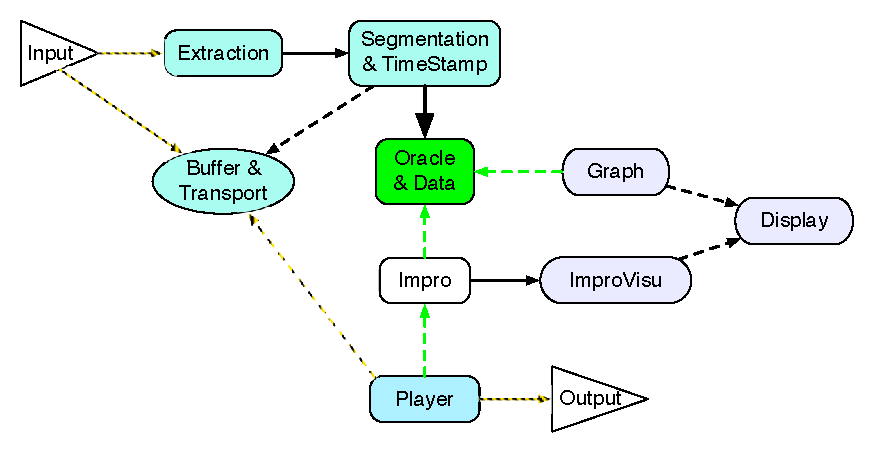
\includegraphics{Modules.eps}
	\caption{Modules of OMax}
	\label{modules}
\end{figure}\\
The \textbf{Extraction} module is in charge of computing the detection information on the input stream. It passes the result to the \textbf{Segmentation \& TimeStamp} module which does the gathering of consistent and sequential description data to constituted the symbolic units and dates them with respect to the recording time. Timestamping is the link between the symbolic units describing the input and the actual recording of the stream made in the \textbf{Buffer \& Transport} module.\\
Then, the symbolic information is organised and stored in the \textbf{Oracle \& Data} module which is thus the core of OMax knowledge. The \textbf{Graph} module periodically reads the model and gives a visualisation of its state which will be displayed by the \textbf{Display} module thanks to Jitter.\\
The \textbf{Impro} module navigates in the knowledge model with respect to the parameters and constraints given through the interface and computes a new path to generate a ``clone''. This path is graphed on the display thanks to the \textbf{ImproVisu} module. Then the \textbf{Player} modules reads this path and with the actual recording recreates a sounding virtual improviser.

%%
\section[The 2.5 worlds of OMax]{The two and a half worlds of OMax\label{2.5worlds}}
OMax 4.x allows two types of input stream of two very different nature: \textbf{MIDI} data coming from a keyboard or any other MIDI instrument or \textbf{audio} coming from a microphone or the reading of a sound file. These two worlds are totally separated in OMax: the bottom half handles the MIDI part (Fig~\ref{midi}) while the top half of the main patch handles the audio part of OMax (Fig~\ref{audio}).
\begin{figure}[h]
	\centering
	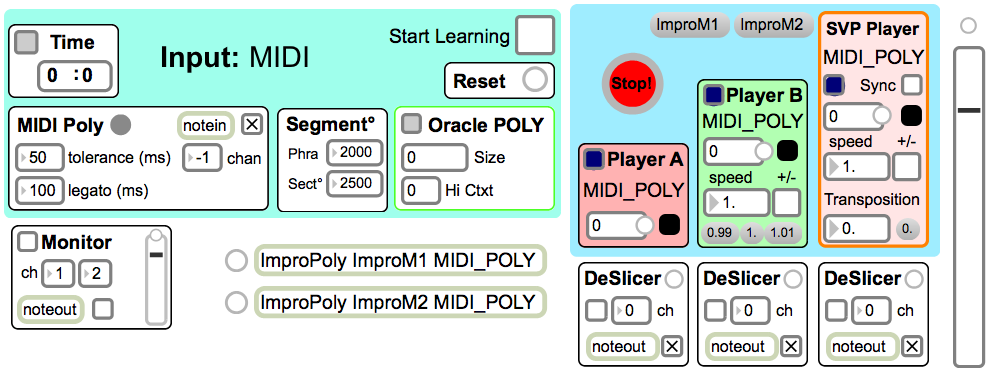
\includegraphics[width=\linewidth]{MIDI.png}
	\caption{MIDI part of OMax}
	\label{midi}
\end{figure}
\begin{figure}[h]
	\centering
	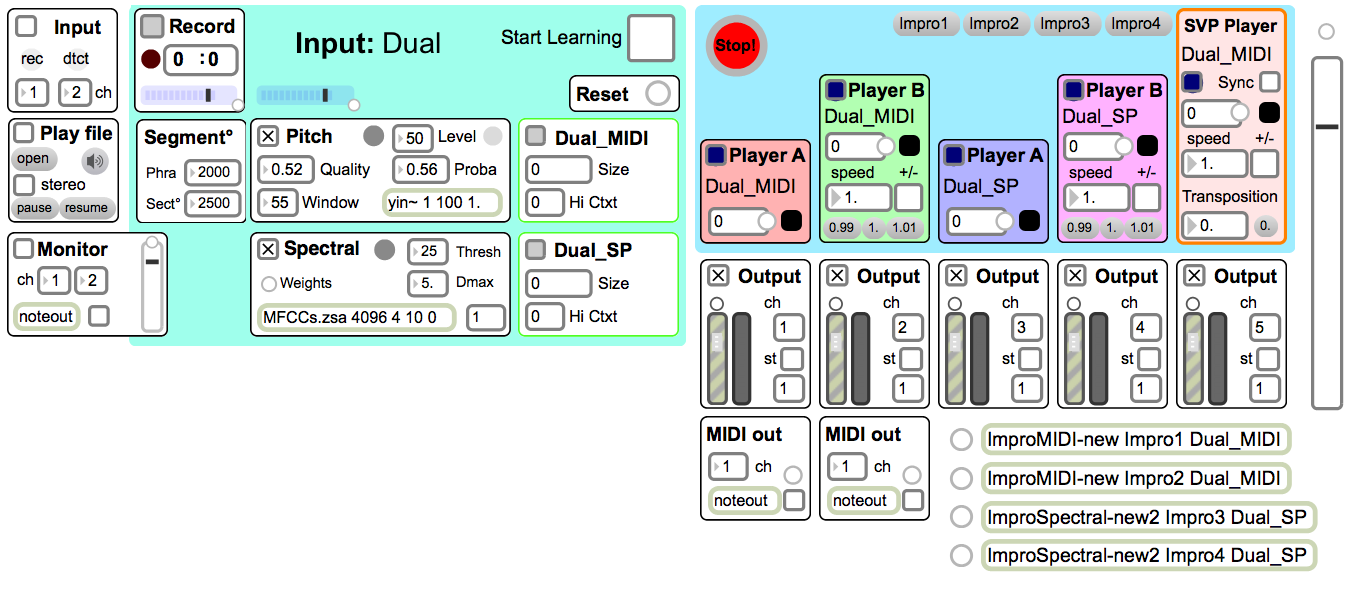
\includegraphics[width=\linewidth]{Audio.png}
	\caption{Audio part of OMax}
	\label{audio}
\end{figure}
\\
Each one of these domain possess its own analysis module(s), data structures and improvisation parts. They share the same conceptual organization presented~\ref{principles} and have the same kind of modules but no link. Only the Jitter display is mutualized for obvious performance and screen reasons.\\
\begin{figure}[h]
	\centering
	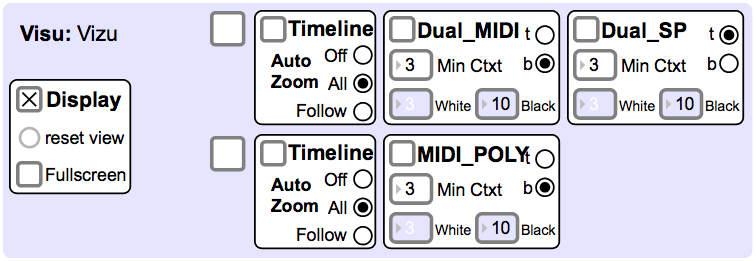
\includegraphics[scale=0.4]{Visu.png}
	\caption{Visualization part of OMax}
	\label{visu}
\end{figure}
%%
\section{Input(s)}
As previously mentioned, there are two types of inputs in OMax and three different analysis possible. We will present here how to use the modules concerning each one of them.
\subsection{MIDI}
The MIDI input of OMax is contained the part of the patch presented Figure~\ref{midiin}. The parameters to get and analyze a MIDI stream are contained in the section framed in red.
\begin{figure}[h]
	\centering
	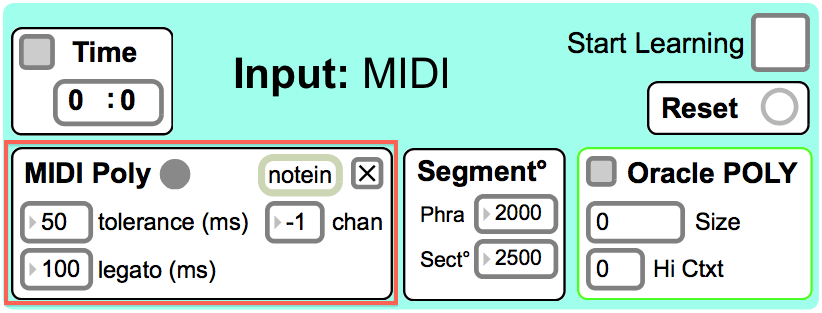
\includegraphics[scale=0.35]{InputMIDI.png}
	\caption{MIDI input section of OMax}
	\label{midiin}
\end{figure}
\begin{description}
	\item[\Ovalbox{\textsf{notein}}~\Ovalbox{\textsf{x}}]: the \textsf{notein} box and its associated toggle is used to select and enable the receiving of MIDI data. Double click on \textsf{notein} to chose the MIDI port.
	\item[\textsf{chan}]: the number labelled \textsf{chan} is used to select a specific MIDI channel to listen to. If the value \verb -1  is put, the data from all the 16 channels of the port will be received.
	\item[\textsf{tolerance}]: the \textsf{tolerance} parameter defines the time granularity (in milliseconds) to separate two MIDI events. Once a note has arrived, all the other notes arriving within the tolerance time will be considered as simultaneous and constituting a common chord. A note arriving after that time will be considered as a new event (possibly a new chord).
	\item[\textsf{legato}]: the legato time (in millisecond) defines the separation between two notes (or chords) that are overlapping. If the overlapping lasts more than the legato time, then the resulting chord is considered as a meaningful event, otherwise, the overlapping is ignored and only the two notes (or chord) before and after are considered.
	\item[\textsf{LED}]: a small grey LED (flashing green) indicates on the right of \textsf{MIDI Poly} if MIDI data arrives in the module.
\end{description}

%
\subsection{Audio}
In the current version of OMax, the analysis being done on an audio stream can rely on two different extractions: \textbf{pitch} content or \textbf{spectral} content. These two analysis run in parallel on the same audio stream so they share the same buffer and timeline but feed to different graphs/knowledge (Factor Oracle) to play with.
The audio input of OMax can come from both a real-time stream of one or two microphones or the playing of a sound file. The modules to adjust the audio input are common for both the pitch or the spectral analysis.
\begin{wrapfigure}{R}{0.5\linewidth}
	\centering
	\vspace{30pt}
	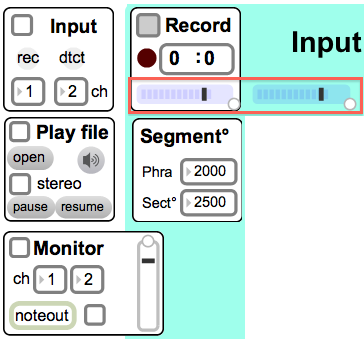
\includegraphics[scale=0.5]{AudioIn1.png}
	\caption{Audio Input of OMax}
	\vspace{20pt}
	\label{audioin}
\end{wrapfigure}
\par
\textsf{\textbf{Input}}: if you have one or two microphones plugged on your computer, you can activate the ``live input'' patch by ticking the toggle on the top left corner and use them. Once you have turned on the DSP of Max/MSP, the two flashing green LEDs named \textsf{\textbf{rec}} (for recording) and \textsf{\textbf{dtct}} (for detection) will tell you if it gets any signal. You can adjust the channel for the recording and the detection separately with the two corresponding number boxes labelled \textsf{\textbf{ch}} (for channel).\\
The detection channel goes into the different extraction and segmentation stages while the recording channel is recorded into the buffer as explained in section~\ref{funct}. It is sometimes better to use two different microphones for those two processes. For example a close field mic, less sensible to the environment (if there are several musicians for instance) may be more efficient for detection while a farther mic will give more bass and air for a better quality recording.\par
\textsf{\textbf{Play file}}: if you want to use a sound file as audio input for OMax, you can use the small player embedded. Start by choosing the file with the \textsf{\textbf{open}} button. Then, once the DSP of Max/MSP is on, checking and unchecking the \textsf{\textbf{toggle}} (top left corner of the \textsf{\textbf{Play file}} frame) starts and stops the playing. You can also \textsf{\textbf{pause}} and \textsf{\textbf{resume}} the playing with the buttons on the bottom of the frame.\\
The \textsf{\textbf{stereo}} toggle lets you choose the routing of the channels if you file is stereo. When uncheck (default), both channels of your file are summed and fed identically into both the detection and recording channels. If you check the \textsf{\textbf{stereo}} toggle, the first channel (left) of your file is fed into the recording while the second (right) is routed to the detection.
\par
Two horizontal \textsf{\textbf{VUmeters}} framed in red on figure~\ref{audioin} are overlaid with two \textsf{\textbf{sliders}} which allows you to adjust the volume of both detection and recording channel. The small \textsf{\textbf{bang}} button at the bottom right corner of each of them is use to come back to the default (127) value. In the \textsf{\textbf{Record}} module, beside seeing and adjusting the recording volume, the red LED let you know when OMax is actually recording and the \textbf{numbers} (refreshed four times per second) indicates the present duration of the recording.
\par
Lastly, the \textsf{\textbf{Monitor}} modules allows you to listen to the audio fed to OMax. You can chose the channel you want to monitor on with the two (one for the recording channel, one for the detection channel) number boxes labelled \textsf{\textbf{ch}} and adjust the volume with the vertical \textsf{\textbf{slider}} on the right (the \textsf{\textbf{bang}} button on top brings back the slider to the default value).

\subsection{Pitch}\label{pitchsection}
Pitch extraction and segmentation are done in the module framed in red on figure~\ref{pitch}.
\begin{figure}[h]
	\centering
	\vspace{12pt}
	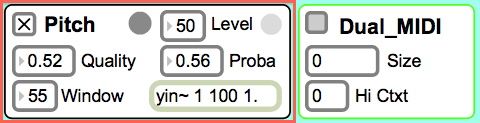
\includegraphics[scale=0.5]{Pitch.png}
	\caption{Pitch detection in OMax}
	\label{pitch}
\end{figure}
\begin{description}
	\item[\textsf{Level}]: to be able to adjust separately the volume of the signal used in the pitch and the spectral detection, you can use the number box labelled \textsf{Level}.
	\item[\textsf{Quality}]: the \Ovalbox{\textsf{yin$\thicksim$}} object outputs along with the pitch stream a \textsf{quality} stream corresponding roughly to the saliency of harmonic frequencies. It is used in OMax as a \textit{relevance} or \textit{consistency} threshold to select dominant pitches. Pitches with a \textsf{quality} under the value given in the number box will be ignored.
	\item[\textsf{Window and Proba}]: a statistical mechanism is included in the pitch detection module to improve the relevance of extracted information. Raw pitches are gathered during a certain time \textsf{window} (in milliseconds) and the so \textit{cooked} pitch is output only if its probability over this window is above the \textsf{Proba} parameter (between 0. and 1.).
\end{description}

%
\subsection{Spectral}\label{spectralsection}
Spectral detection in OMax relies on descriptors named MFCCs for Mel-frequency cepstral coefficients.
% More details about the functioning are given~\ref{specdetails}. 
If you do not want to use presets supplied with the patch, you can adjust manually the parameters shown in the red frame of figure~\ref{spectral}.
\begin{figure}[h]
	\centering
	\vspace{12pt}
	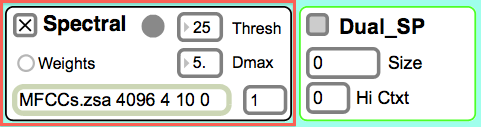
\includegraphics[scale=0.5]{Spectral.png}
	\caption{Spectral detection in OMax}
	\label{spectral}
\end{figure}
\begin{description}
	\item[\textsf{Thresh}]: the first coefficient of MFCCs represent the overall energy of the spectrum. As with quality in pitch, we can exclude spectral slices of too weak energy (as background noises for example) with the \textsf{Thresh} number box. The higher you put this threshold, the less sensible the detection will be.
	\item[\textsf{Dmax}]: an adaptive clustering is implemented in this detection to recognize similar pitches% (see~\ref{specdetails} for more)
. It uses a distance to compare the spectral content of the frames. The \textsf{Dmax} parameter adjusts the maximal distance for two frames to be considered as similar. Practically, it means that if you decreasing Dmax you gives the detection a finer resolution (differentiation) but may drastically decrease the quality of recognized patterns in the model as well. Increasing Dmax will agglomerate more different spectral contours as one type of spectrum which may augment the number of recognized patterns in the model but lower their relevancy.
\end{description}


%
\subsection{Common interfaces}
\subsubsection{Silence segmentation}
\begin{wrapfigure}[4]{R}{0.33\linewidth}
	\centering
	\vspace{-20pt}
	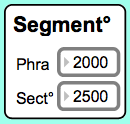
\includegraphics[scale=0.5]{Seg.png}
	\caption{Silence segmentation}
	\label{seg}
\end{wrapfigure}
For both MIDI and audio input, OMax also performs a two level higher scale segmentation based on silences.
The input stream is cut into phrases and sections based on the durations (in milliseconds) given in the number boxes labelled \textsf{\textbf{Phra}} and \textsf{\textbf{Sect�}}.
\vspace{1em}
\subsubsection{Current state of the model}
Lastly, each detection gives you a feedback (presented figure~\ref{oracles}) on the current state of the model once you have started the learning (see~\ref{quick} to learn how to start). \textsf{\textbf{Size}} indicates the number of states in the Factor Oracle graph ie. the number of elements in OMax knowledge model of the input sequence. And \textsf{\textbf{Hi Ctxt}} (for highest context) displays the length of the longest repeated pattern recognized in the model. This gives you a clue on the current state of the learning and also some information on the adjustment of the detection. Typical values for highest context should be above 3 and not higher than 15 except if the source itself has some long repetitions.
\begin{figure}[h]
	\centering
	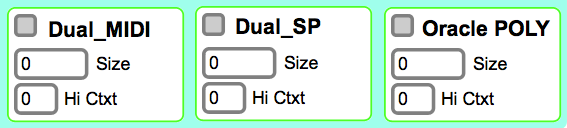
\includegraphics[scale=0.5]{Oracles.png}
	\caption{Current state of the Factor Oracle}
	\label{oracles}
\end{figure}

%%
\newpage
\section{Improvisation(s)}
The improvisation part of OMax strongly relies on the Factor Oracle model used to analyze the source material~(see~\ref{principles}). Variations or ``clones'' played by OMax are created by navigating this model and jumping from time to time to diverge from the original material. While the principle of this navigation are common to the different inputs and analysis done in OMax (see~\ref{2.5worlds}) some specialization are needed to adapt the result to the different material and gain in smoothness and musicality.
\subsection{Core}\label{core}
\begin{wrapfigure}{R}{0.6\linewidth}
	\centering
	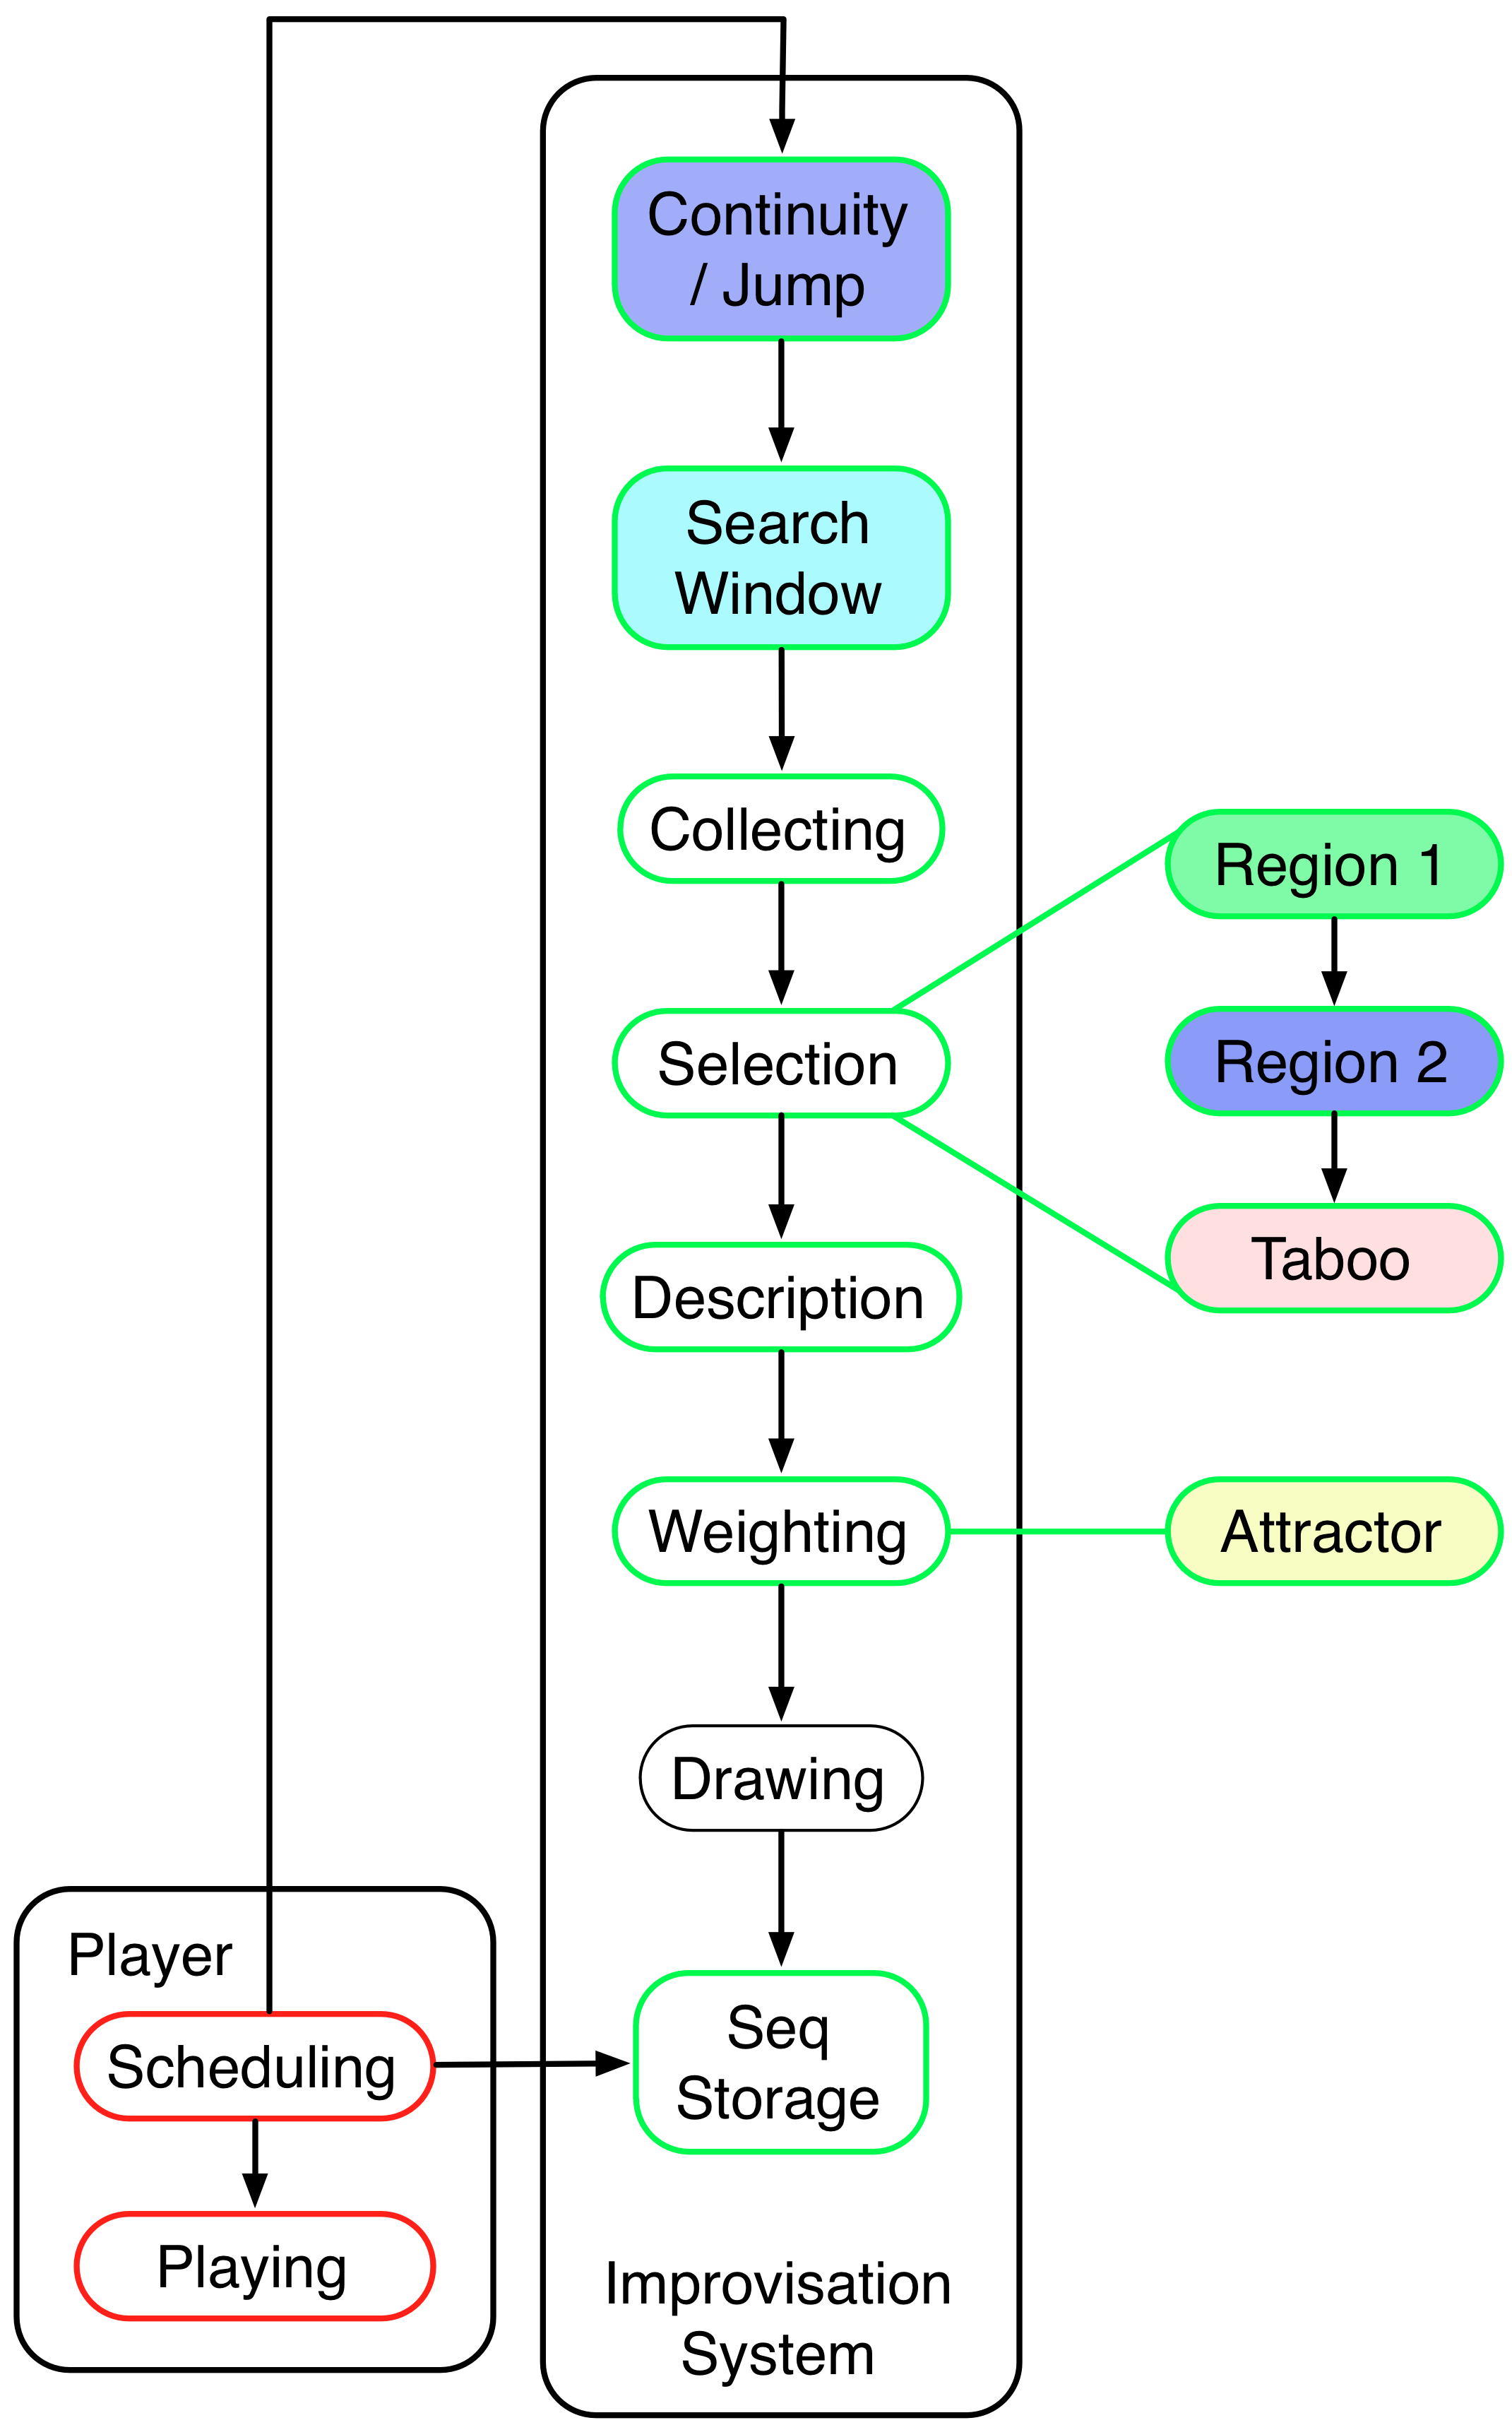
\includegraphics{Impro.png}
	\caption{Improvisation \& Player System}
	\label{impro}
\end{wrapfigure}
%The common navigation strategy to create OMax improvisations has been described in \ref{Navigation the Oracle}. 
In OMax 4.x the navigation strategy follows the functional diagram presented opposite (figure~\ref{impro}).\\
The original sequence is read for a few consecutive elements (ie a few notes or a short duration) that we name \textbf{continuity} then, it is time to diverge from the original sequence and the system decides to \textbf{jump}.\\
OMax has a small anticipation system to be able to find a good transition (variation) so it searchs and \textbf{collects} the different solutions over a short \textbf{searching window}.\\
It \textbf{selects} next all these solutions based on different criteria both automatic (as a \textbf{taboo} system to avoid strict loops) and user based (as \textbf{regions} which allow to choose the part of the past serving as source). And discards solutions not following these rules.\\
Remaining solutions are \textbf{described} musically with parameters which strongly depends on the type of analysis and each solution is \textbf{weighted} with a mixture of these parameters. So the pool of solutions is ordered according to this weight.\\
Finally, one of the solution is \textbf{drawn} (among the best), validated and planned as the next jump. The destination of this jump starts a new continuous sequence and buckles the cycle.\\
\smallskip
\\
Interface for this common mechanism is presented figure~\ref{improinterface}.
There are six of these improvisation core in the current version of OMax. Four of them are attached to the audio input (Fig~\ref{boxaudio}), two of them deal with MIDI data (Fig~\ref{boxmidi}). You can open and interact with them by double-clicking on their box (showed figure~\ref{boxes}).\\
\begin{figure}[h]
	\centering
	\subfloat[Audio improvisation boxes]{\label{boxaudio}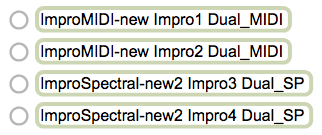
\includegraphics[width=0.4\linewidth]{ImproPatches.png}}
	\subfloat[MIDI improvisation boxes]{\label{boxmidi}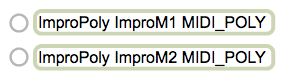
\includegraphics[width=0.36\linewidth]{ImproPatches2.png}}
	\caption{Improvisation cores boxes}
	\label{boxes}
\end{figure}\\
Each one of these core is reading and improvising on one type of analysis only, indicated by the second argument given to these boxes. \textsf{Dual\textunderscore MIDI} stands for pitch description, \textsf{Dual\textunderscore SP} stands for spectral description (\textsf{Dual} being the name of the audio input) and \textsf{MIDI\textunderscore POLY} is the model of the MIDI input.\\
\begin{figure}[h]
	\centering
	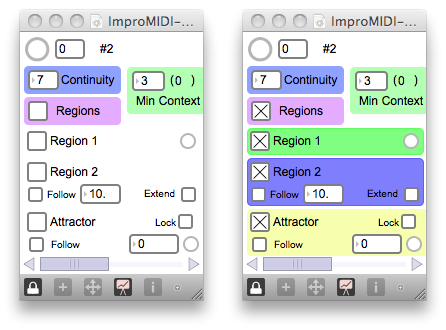
\includegraphics[scale=0.7]{ImproInterface.png}
	\caption{Common Improvisation Interface}
	\label{improinterface}
\end{figure}
\begin{description}
	\item[\textsf{Continuity}]: acts as a kind of \textit{variation rate}. The higher, the longer consecutive chunks will be (so the lesser OMax will diverge from the original material). \\\danger~Typical value for \textsf{continuity} strongly depends on the type of analysis.
	\item[\textsf{Min Context}]: acts as a kind of \textit{smoothness} parameter. The higher, the smoother divergences from the original material will be. However, forcing higher contexts makes also possibilities of jumps rarer. In brackets is recalled the highest context currently found in the model% (see~\ref{factororacle} for more)
.\\ \danger~Putting a higher value than the one in brackets will stop OMax to vary from the original.
	\item[\textsf{Regions}]: this toggle globally activate or deactivate the \textsf{region} mechanism. Defining the regions is done either directly on the visualization (see~\ref{selection}~\S 2) or automatically with the \textsf{follow} or \textsf{extend} mode in the case of \textsf{region 2} (see \textsf{region 2} below).
	\item[\textsf{Region~1}]: enables and disables the \textsf{first region} shown in green on the visualization.
	\begin{description}
		\item[\textsf{Button}]: the bang on the right of \textsf{Region 1} line sends the reference of the middle of green region to the attractor. 
	\end{description}
	\item[\textsf{Region~2}]: enables and disables the \textsf{second region} appearing in blue on the visualization.
	\begin{description}
		\item[\textsf{Follow}]: besides selecting manually (see~\ref{vizu}) 
the \textsf{region 2}, you can have it automatically set to the last $x$ seconds --~$x$ being set by the \textsf{number box} next to the \textsf{Follow} word~-- by ticking the \textsf{Follow} box.
		\item[\textsf{Extend}]: like the \textsf{Follow} (but exclusively with it), right bound of \textsf{region 2} can be set automatically to the most recent event learnt in OMax while the left bound is set by the user. This allow to have a \textsf{second region} extending towards the present but limited in the past.
	\end{description}
	\item[\textsf{Attractor}]: aside from regions that are strict constrains, an attractor can be placed on the timeline (see~\ref{vizu}) 
to help OMax ``clone'' to vary around a specific element of the past. The main \textsf{toggle} (next to the word \textsf{Attractor}) activate and deactivate this effect. The \textsf{number box} allows to place it. \\ \danger~Range for the attractor goes from 0 to the most recent event learnt which depends of course from the input and the analysis.
	\begin{description}
		\item[\textsf{Follow}]: automatically puts (and updates) the \textsf{Attractor} to the most recent event learnt.
		\item[\textsf{Lock}]: is useful when the attractor position has been set through \textsf{Region 1}. If you activate the \textsf{Attractor} with \textsf{Lock} ticked, the attractor will help the ``clone'' to get inside the green region. As soon as it is inside, the \textsf{Attractor} will be replaced by the \textsf{Region 1}. The effect is a smoother (but longer) transition of the ``clone'' to get into \textsf{Region 1} thanks to the \textsf{Attractor}.
	\end{description}
\end{description}

%
%\newpage	
\subsection{Players}
Core patches presented in the previous paragraph (\ref{core}) generates improvised sequence however they do not play them. Players, located in the right half of the main OMax patch are in charge of effectively playing the ``clones''.
%\bigskip
\par
There are five players for the audio part of OMax (Figure~\ref{audioplayers}) and three for the MIDI part (Figure~\ref{midiplayers}). There are also three types of players in OMax: players of \textbf{type A}, players of \textbf{type B} and \textbf{SVP} players.\\
In the default configuration of OMax, each player, except SVP players, is reading (and polling) a different improvisation core. For example in the audio part, the first player on the left (red) is reading the first improvisation core (named Impro1 and navigating the pitch description,  \textsf{Dual\textunderscore MIDI}, of the input), the second player (green) reads Impro2, the third (blue) reads Impro3 (navigating on \textsf{Dual\textunderscore SP}, the spectral description of the input) and the fourth (magenta) reads Impro4 core. The players color matches the color of the core being read.\\
The same thing is also true for the MIDI part: the first player reads the first improvisation core (named ImproM1, in red) and the second player reads the ImproM2 improvisation core (in green).
%\smallskip
\par
\textbf{SVP players} are versatile and can read indiscriminately any improvisation core (of the same input). You can switch from one core to another with the message on the top labelled with the name of the cores: \textit{Impro1, Impro2, Impro3, Impro4} for the audio part and \textit{ImproM1 and ImproM2} for the MIDI part.
\begin{figure}[h]
	\centering
	\subfloat[Audio Players]{\label{audioplayers}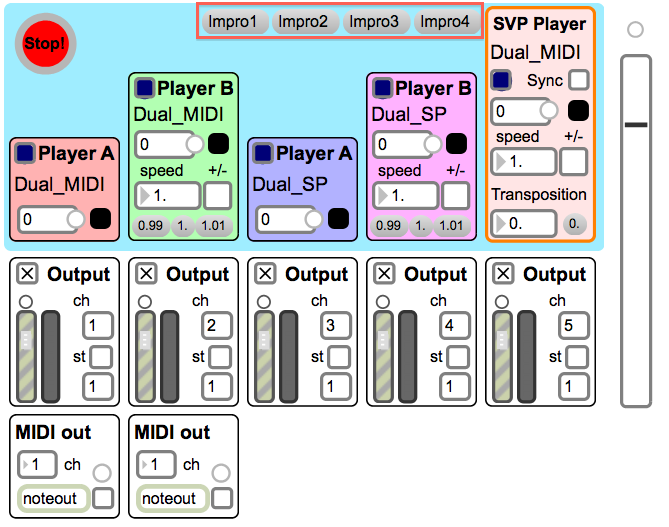
\includegraphics[scale=0.37]{PlayersAudio.png}}
%	\\ \smallskip
\hspace{1em}
	\subfloat[MIDI Players]{\label{midiplayers}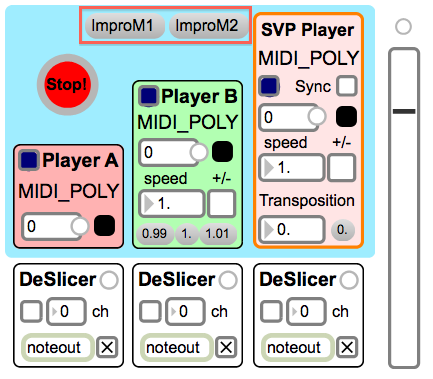
\includegraphics[scale=0.37]{PlayersMIDI.png}}
	\caption{Players}
	\label{players}
\end{figure}
\par
\subsubsection{Player A}
\begin{wrapfigure}[6]{L}{0.23\linewidth}
	\centering
	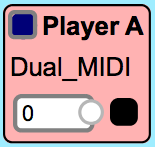
\includegraphics[width=0.7\linewidth]{PlayerA.png}
	\caption{Player A}
	\label{playerA}
\end{wrapfigure}
Players of type A are the simplest player possible. They start and stop with the \textbf{toggle} in their top left corner (on a dark blue background). The background of this toggle flashes (with a light blue color) whenever a variation (from the learnt input) occurs. The \textbf{number} indicates how many states (notes, chords or spectral slices) has already been read. And the \textbf{black button} on the right of the number box lets the player find a smooth ending then stop there.
\vspace{3em}
\par
%\newpage
\subsubsection{Player B}
\begin{wrapfigure}[11]{L}{0.23\linewidth}
	\centering
	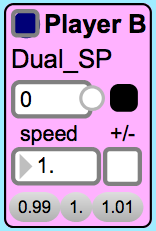
\includegraphics[width=0.7\linewidth]{PlayerB.png}
	\caption{Player B}
	\label{playerB}
\end{wrapfigure}
Players of type B works the same way as players of type A: start and stop \textbf{toggle} is in the top left corner on a blue background, flashing when a variation occurs. The \textbf{number} indicates the size of the sequence already played and the \textbf{black button} triggers a smooth ending.\\
Besides these basic functions, players of type B provides a variable speed option. The \textbf{floating-point} speed \textbf{box} is a multiplicative factor going from $5.$ to $-5.$ Normal speed is $1.$, $2.$ means two times faster, $0.5$ half the normal speed (ie. two times slower) and so on. Negative speeds automatically ticks the \textbf{toggle} box labelled \textit{+/-} and means reading the sound backward. However these changes of speed are link with a ``natural'' transposition exactly as when rotating old vinyls faster or slower.
\vspace{1em}
\par
\subsubsection{SVP Player}
\begin{wrapfigure}{R}{0.23\linewidth}
	\centering
	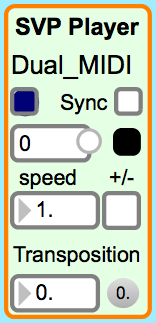
\includegraphics[width=0.7\linewidth]{PlayerSVP.png}
	\caption{Player SVP}
	\label{playerSVP}
\end{wrapfigure}
SVP players make use of the Super Phase Vocoder developed at IRCAM and allows on top of the regular functions of the other players to transpose and/or change the speed independently. Start/stop \textbf{toggle}, smooth ending \textbf{button} and speed \textbf{box} work exactly as in Players of type B. Another \textbf{floating-point number box} allows to transpose finely the whole clone from 18 semi-tones below to 18 semi-tones above the original tuning (a value of $1.$ meaning one semi-tone above).\\
A SVP player can also be synchronized on another player (of type A or B) and thus used to harmonize a clone with a transposition for example. You need first to choose on which of the other players you want to synchronize with the buttons labelled \textit{Impro1\dots4} (or \textit{ImproM1\dots2} in the case of MIDI section) framed in red on Figure~\ref{players}. Then you can tick the \textit{Sync} \textbf{toggle} to synchronize the SVP player. You can check that they are indeed well synchronized by watching the \textbf{number box} showing the state being read.
\subsubsection{Output}
\begin{wrapfigure}[15]{L}{0.23\linewidth}
	\vspace{-2em}
	\centering
	\subfloat[Audio Output]{\label{audioout}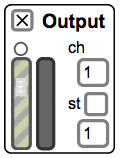
\includegraphics[width=0.7\linewidth]{AudioOut.png}}\\
%	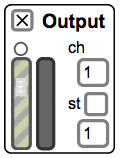
\includegraphics[width=0.15\linewidth]{AudioOut.png}
\smallskip
	\subfloat[MIDI Output]{\label{midiout}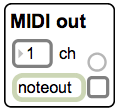
\includegraphics[width=0.7\linewidth]{MIDIout.png}}
	\caption{}
	\label{out}
\end{wrapfigure}
\vspace{1em}
Below each of the players, you will find a small audio output patch which will let you adjust the volume with the left-hand side \textbf{fader}. The \textbf{view meter} lets you know the loudness of the clone (before applying the volume of the fader). You can choose the channel (\textit{ch}) with the top \textbf{number box} on the right-hand side and decide to duplicate the output to another channel by ticking the stereo (\textit{st}) \textbf{toggle} and addressing another channel with the second \textbf{number box}. You may also deactivate the whole audio output of the clone with the top left \textbf{toggle}.\\[1em]
This is useful in the case of a ``clone'' on the pitch description. Indeed this description of the audio input is able to emulate a monophonic MIDI stream. You can then play the ``clones'' through MIDI with the patch presented Figure~\ref{midiout}. Enable the MIDI playback by ticking the \textbf{toggle} next to the \textsf{noteout} box of the \textit{MIDI out} patch. Choose the channel (\textit{ch}) with the \textbf{number box} and the MIDI destination by double clicking on the \textsf{noteout} box. Use the \textbf{button} on the right to flush all MIDI notes.\\
\vspace{4em}
\par
\begin{wrapfigure}[7]{R}{0.23\linewidth}
	\vspace{-1em}
	\centering
	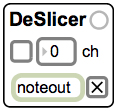
\includegraphics[width=0.7\linewidth]{Deslicer.png}
	\caption{}
	\label{deslicer}
\end{wrapfigure}
In the case of the MIDI part of OMax, the output is named \textit{DeSlicer}% (see~\ref{slicing})
. It lets you choose the destination of the MIDI stream by double clicking on the \textsf{noteout} box which may be deactivated with the \textbf{toggle} on its right. By default, the output of MIDI OMax uses the same channel(s) as the input stream it learnt but you can override this by choosing a channel with the \textbf{number box} labelled \textit{ch} and ticking the \textbf{toggle} on its left. The \textbf{button} in the top right corner flushes (ie. stops) all the MIDI notes on every channel.
%%
\vspace{1em}
\section{Visualisation}
Version 4.x has added a novel visualization to OMax. The state of the internal knowledge (Factor Oracle) can be represented in real time thanks to Jitter (the graphical part of MaxMSP), see Figure~\ref{vizuregions} for an example. There is only one (jitter) rendering window (named \textsf{Vizu}); as a result, you can display only one timeline (ie. one of the two inputs ---~Audio or MIDI~--- of OMax) at a time. However, when visualizing the audio input, both pitch and spectral modelling can be represented above and below the timeline.
\begin{figure}[h]
	\centering
	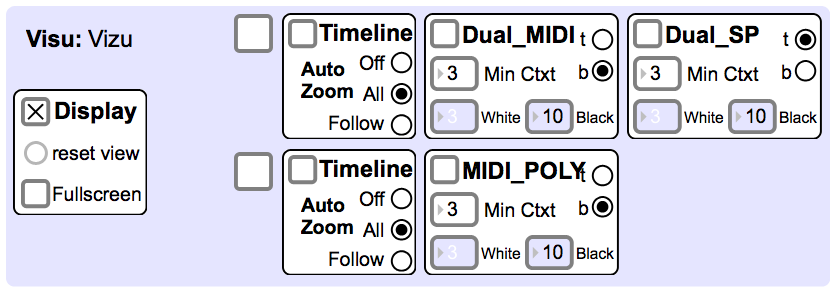
\includegraphics[scale = 0.35]{Vizu.png}
	\caption{Visualization Control Interface}
	\label{vizu}
\end{figure}
\subsubsection{Display}
\begin{wrapfigure}[5]{L}{0.23\linewidth}
	\vspace{-1em}
	\centering
	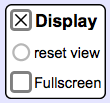
\includegraphics[width=0.7\linewidth]{Display.png}
	\caption{}
	\label{display}
\end{wrapfigure}
\vspace{1em}
The \textsf{Display} module is in charge of refreshing and handling the Jitter window. You can start and stop computing the graphics with the \textbf{top left toggle}.
The \textbf{button} labelled \textsf{reset view} re-centres the view on the default origin of the display.
Finally, you can put the visualization fullscreen with the \textbf{bottom left toggle}. Press the \textit{Esc} key to come back to the window mode.
\vspace{2em}
\subsubsection{Timeline}\label{line}
\begin{wrapfigure}{R}{0.23\linewidth}
	\centering
	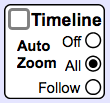
\includegraphics[width=0.7\linewidth]{Timeline.png}
	\caption{}
	\label{timeline}
\end{wrapfigure}
The \textsf{Timeline} module allows to show an horizontal line representing the elapsed time of recording and learning (growing in realtime). The \textbf{toggle} enable and disable this rendering. This module is also in charge of adjusting the zoom of the display. If you turn the \textsf{Auto Zoom} function \textit{Off} with the first option of the \textbf{radio button} on the right, the display will simply stay still as it was. Clicking on the \textit{All} option or pressing the \textit{spacebar} of your keyboard will set (and automatically refresh) the zoom to display the whole knowledge. The \textit{Follow} option will slide the display horizontally towards the right as the learning is growing.
\par
\label{selection}
Along the timeline and thanks to the \textsf{Display} module ---~which is also in charge of converting the mouse position into time position in the recording~--- you can select regions (region 1 in green, region 2 in blue) on the visulization. Simply click, hold and release the mouse to extend the region 1. Defining a region 2 works the same way with the \textsf{shift} key pressed while selecting. Depending whether you selected a region above or below the timeline, this region will refer to (and be used to control) the pitch or the spectral model (see~\ref{linkssection}, radio button).
\subsubsection{Links}\label{linkssection}
\begin{figure}[h]
	\centering
	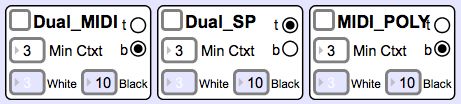
\includegraphics[scale = 0.60]{VizuLinks.png}
	\caption{Control of the visualization of the links}
	\label{links}
\end{figure}
The main visual information about the state of the model is given by tracing the links of the graph. This is controlled, for each graph being built, with the interface presented above (Fig~\ref{links}). The \textbf{toggle} enable and disable this function, the \textbf{radio button} on the right of the box controls if the links (for each graph) is displayed above (\textit{t} for top) or below (\textit{b} for bottom) the horizontal timeline (see~\ref{line}). You can choose the minimal quality of links to render with the \textbf{number box} labelled \textsf{Min Ctxt}, a higher value will display fewer but better quality links (and may allow you to save some CPU). The quality (context length) of the links are shown with a grey scale going from white (lower contexts) to black (higher contexts). Changing the \textsf{Min Ctxt} value will also set the \textsf{White} \textbf{number box} to the same value adjusting this way the grey scale to your display. However, you can also change these parameters by hand by indicating in the \textsf{Black} and \textsf{White} \textbf{number boxes} your bounds for the grey scale. It may be useful if you want to project the visualization on a large screen or if you work in specific lights conditions which dims the differences in colors.
\par
\begin{figure}[h]
	\centering
	\subfloat[Full Audio Visualization]{\label{viztog1}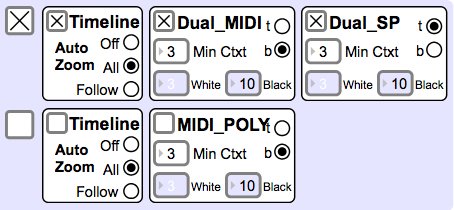
\includegraphics[width=0.485\linewidth]{VizuTog1.png}}
	\hspace{0.8em}
	\subfloat[Full MIDI Visualization]{\label{viztog2}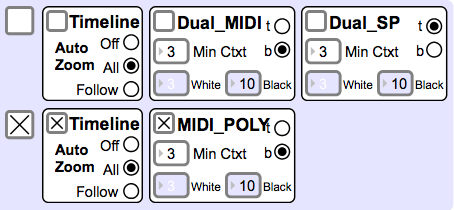
\includegraphics[width=0.485\linewidth]{VizuTog2.png}}
	\caption{Toggle Shortcut for Visualization}
	\label{vizutog}
\end{figure}
A handy shortcut is provided in the interface to activate/deactivate all the features at once. The \textbf{bigger toggle} on the left of the \textsf{Timeline} boxes will check all the other boxes of the same row. Because there is only one Jitter rendering window, both bigger toggles are mutually exclusive so that you can visualize the two models built on the Audio input \textbf{or} the model built on the MIDI input but not both.\\
%\begin{figure}[h]
%	\centering
%	\centerline{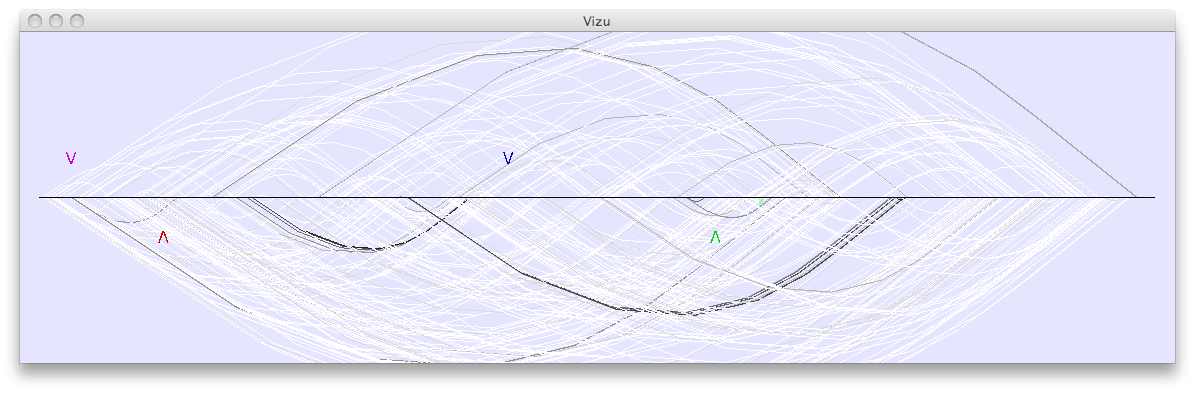
\includegraphics[width=1.\linewidth]{VizuWin.png}}
%	\caption{Example of the Visualization Window}
%	\label{vizuwin}
%\end{figure}
\begin{figure}[h]
	\centering
	\centerline{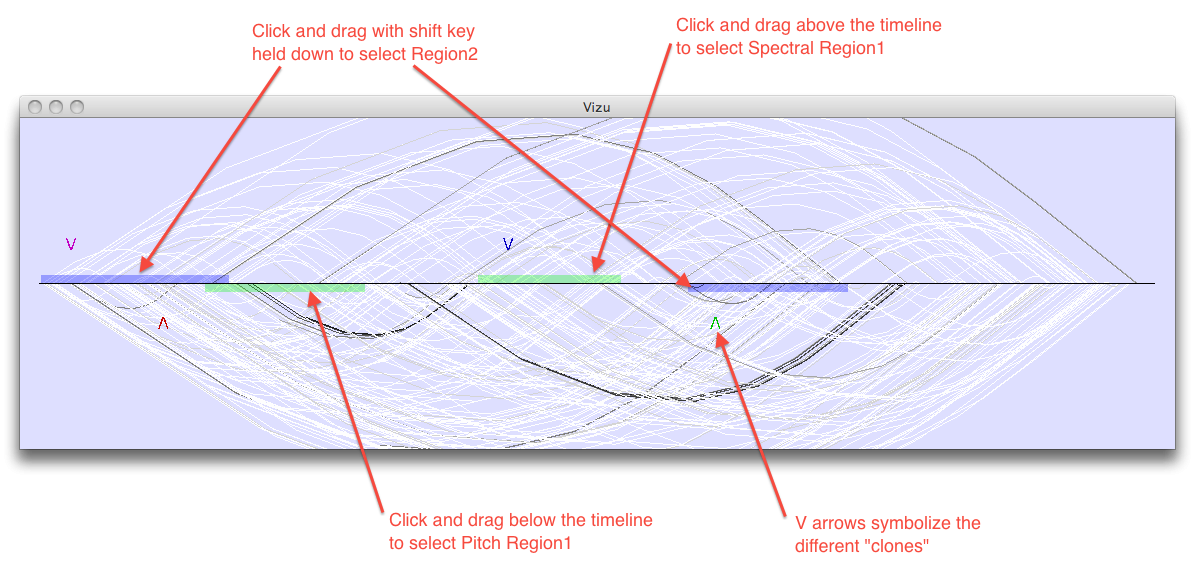
\includegraphics[width=1.\linewidth]{VizuRegions2.png}}
	\caption{Example of the Visualization Window with Regions}%\vspace{1em}\\ Everything concerning spectral description is drawn above the timeline,\\ everything concerning pitch description is shown below the timeline.}
	\label{vizuregions}
\end{figure}

%
%%%%%%%%%%%%%%%%%%%%%
\chapter{Advanced Usage}
This section presents more advanced features of OMax 4.5.x. It assumes that you are comfortable enough with Max/MSP so that you know how to edit a patch, switch between presentation and edit mode, use the embedded help on inlets and outlets and the inspector, know the concepts of objects, abstractions or bpatchers and other basic Max/MSP functions.

\section{Controling OMax with Messages}
The inputs (inlets) and outputs (outlets) of all the modules of OMax are documented in the patch. That means that if you mouse over any inlet/outlet it will display information on the purpose of this inlet/outlet. You can use those inlets at your convenience to interact directly with any module with Max messages (and toggles etc.) instead of using the graphical interface. Most of the inlets correspond to parameters described earlier in this documentation. For example, Figure~\ref{inlet-help} shows the first (left-most) inlet of the Player A (see~\ref{playerA}) which is used to start and stop the ``\,clone\,''.	
\begin{figure}[!h]
	\centering
	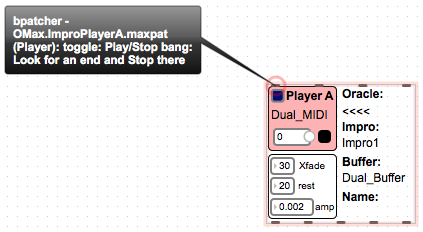
\includegraphics[width=0.6\linewidth]{Inlet-Help.png}
	\caption{Example of an inlet and its help}
	\label{inlet-help}
\end{figure}\\
Few inlets though are used for purposes that are not previously described. The embedded info should be self-explanatory or this inlet is not controlling any user-level parameter and you should not use it either. The last (right-most) inlet of every module (either loaded as an abstraction or in a bpatcher) which includes settable parameters is always named \textbf{patterhub}. It is used to access and change all the parameters of the module even if some of them are not shown in the graphical interface.
\begin{figure}[!h]
	\centering
	\subfloat[abstraction]{\label{abstraction}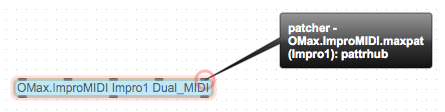
\includegraphics[scale=0.45]{pattrhub.png}}
%	\\ \smallskip
\hspace{1em}
	\subfloat[bpatcher]{\label{bpatcher}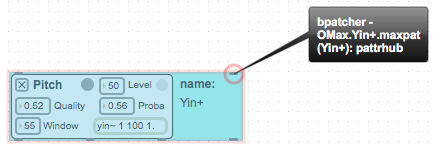
\includegraphics[scale=0.45]{pattrhub2.png}}
	\caption{pattrhub inlet (right-most)}
	\label{pattrhub}
\end{figure}
Figure~\ref{pattrhub} shows this inlet for the Improvisation core module (see~\ref{core}) which is loaded as an abstraction (Figure~\ref{abstraction}) and for the Pitch extraction module (Figure~\ref{bpatcher}, see~\ref{pitchsection}) which is loaded in a bpatcher. This inlet allows to send direct messages to the module with the name of a parameter (even if the parameter is hidden in the graphical interface) and a value to assign to this parameter.
\par
\begin{wrapfigure}[8]{L}{0.4\linewidth}
	\centering
	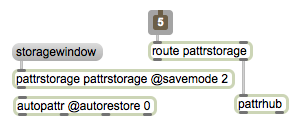
\includegraphics[width=0.9\linewidth]{pattrsystem.png}
	\caption{}
	\label{pattrsystem}
\end{wrapfigure}
This mechanism relies on the \textbf{pattr} system of Max/MSP. Figure~\ref{pattrsystem} shows the simple set of \textbf{pattr} objects used in every module. If you double-click on the \textbf{pattrstorage} object, a list of all the parameters accessible in the module you are exploring will pop-up. As explained in the documentation of the \textbf{pattrstorage} object, this \textit{Client Objects} list reflects the state of all the parameters watched by the pattr system. If you change any parameter either with the graphical interface or with a message, the current value of that parameter will be reflected in this window as well. This way, it is very easy to link a parameter to the corresponding name in the pattr system and know which message to send in the \textbf{pattrhub} inlet of the module. Figure~\ref{pattrstorage-messages} shows an example of such control of the Improvisation core module (see~\ref{core}) with a few messages and the associated list of parameters.
\begin{figure}[!h]
	\centering
	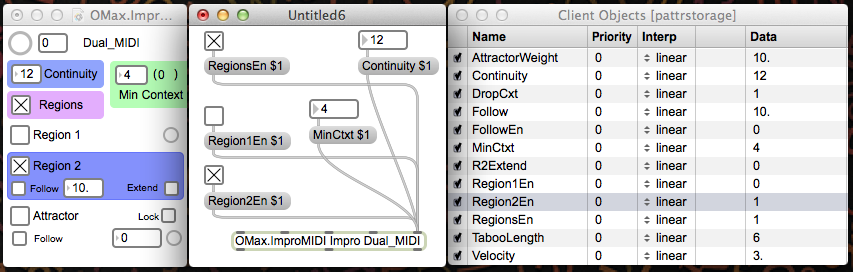
\includegraphics[width=\linewidth]{pattrstorage-messages.png}
	\caption{Example of an interaction through messages to the pattr system of the Improvisation core}
	\label{pattrstorage-messages}
\end{figure}\\

\subsubsection{Regions}
Aside from the pattrhub system, there are messages received in the \textbf{Selections} subpatcher (Figure~\ref{selections}) to remotely set the regions used to control the location of the ``\,clones\,''. The boundaries of the regions should be sent using the number of the state in the model for the beginning and end of each region. This pair of integer is to be sent to \textbf{Dual\_MIDI-selection1} or \textbf{Dual\_MIDI-selection2} for the regions of the pitch description, \textbf{Dual\_SP-selection1} or \textbf{Dual\_SP-selection2} for the regions on spectral description or \textbf{MIDI\_POLY-selection1} or \textbf{MIDI\_POLY-selection2} for the regions of the MIDI input.
\begin{figure}[!h]
	\centering
	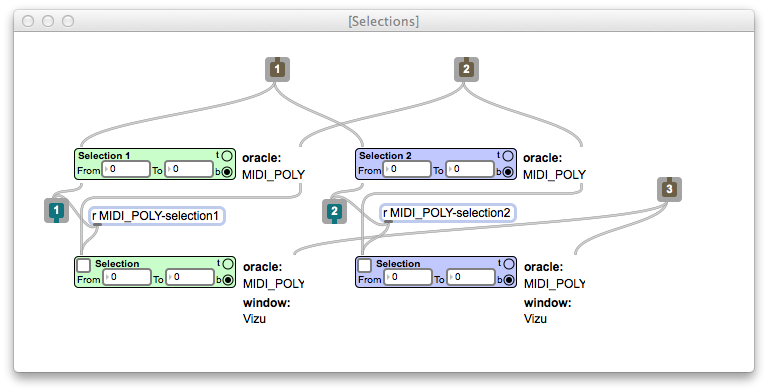
\includegraphics[width=0.9\linewidth]{Selections.png}
	\caption{Receive objects to remotely set regions (presented here for the MIDI input)}
	\label{selections}
\end{figure}\\
To convert from time to state number in any of the models, you can use the \textbf{OMax.date2state} external object which takes as argument the name of the model you want to refer to. You can also use the elapsed recording time (that is the most recent date along the timeline of the learning) which is output from the right outlet of the \textbf{OMax.Buffer} module (for the audio input) or the \textbf{OMax.Time} module (for the MIDI input) as shown Figure~\ref{elapsed}.
\begin{figure}[!h]
	\centering
	\subfloat{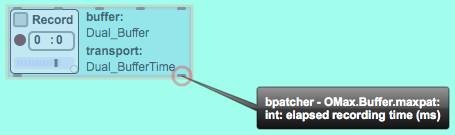
\includegraphics[width=0.6\linewidth]{OMax-Buffer.png}}
	\\
%\vspace{1em}
	\subfloat{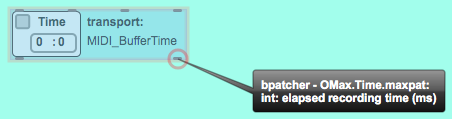
\includegraphics[width=0.6\linewidth]{OMax-Time.png}}
	\caption{Elapsed Time Output}
	\label{elapsed}
\end{figure}

\section{References Through Names}
\subsection{Names}
There are in OMax 4.5.x a few absolute names which constitute univocal references to underlying data structures as the audio buffer, the internal model (see~\ref{overview}), the jitter window of the visualization part etc. The names are declared to Max/MSP when loading the OMax patch and can not be changed afterward without closing it. Therefore they will be conflicts if you load two times the main OMax 4.5.x for example. The architecture of the names (except for the visualization part) is illustrated Figure~\ref{names}.
\begin{figure}[!h]
	\centering
	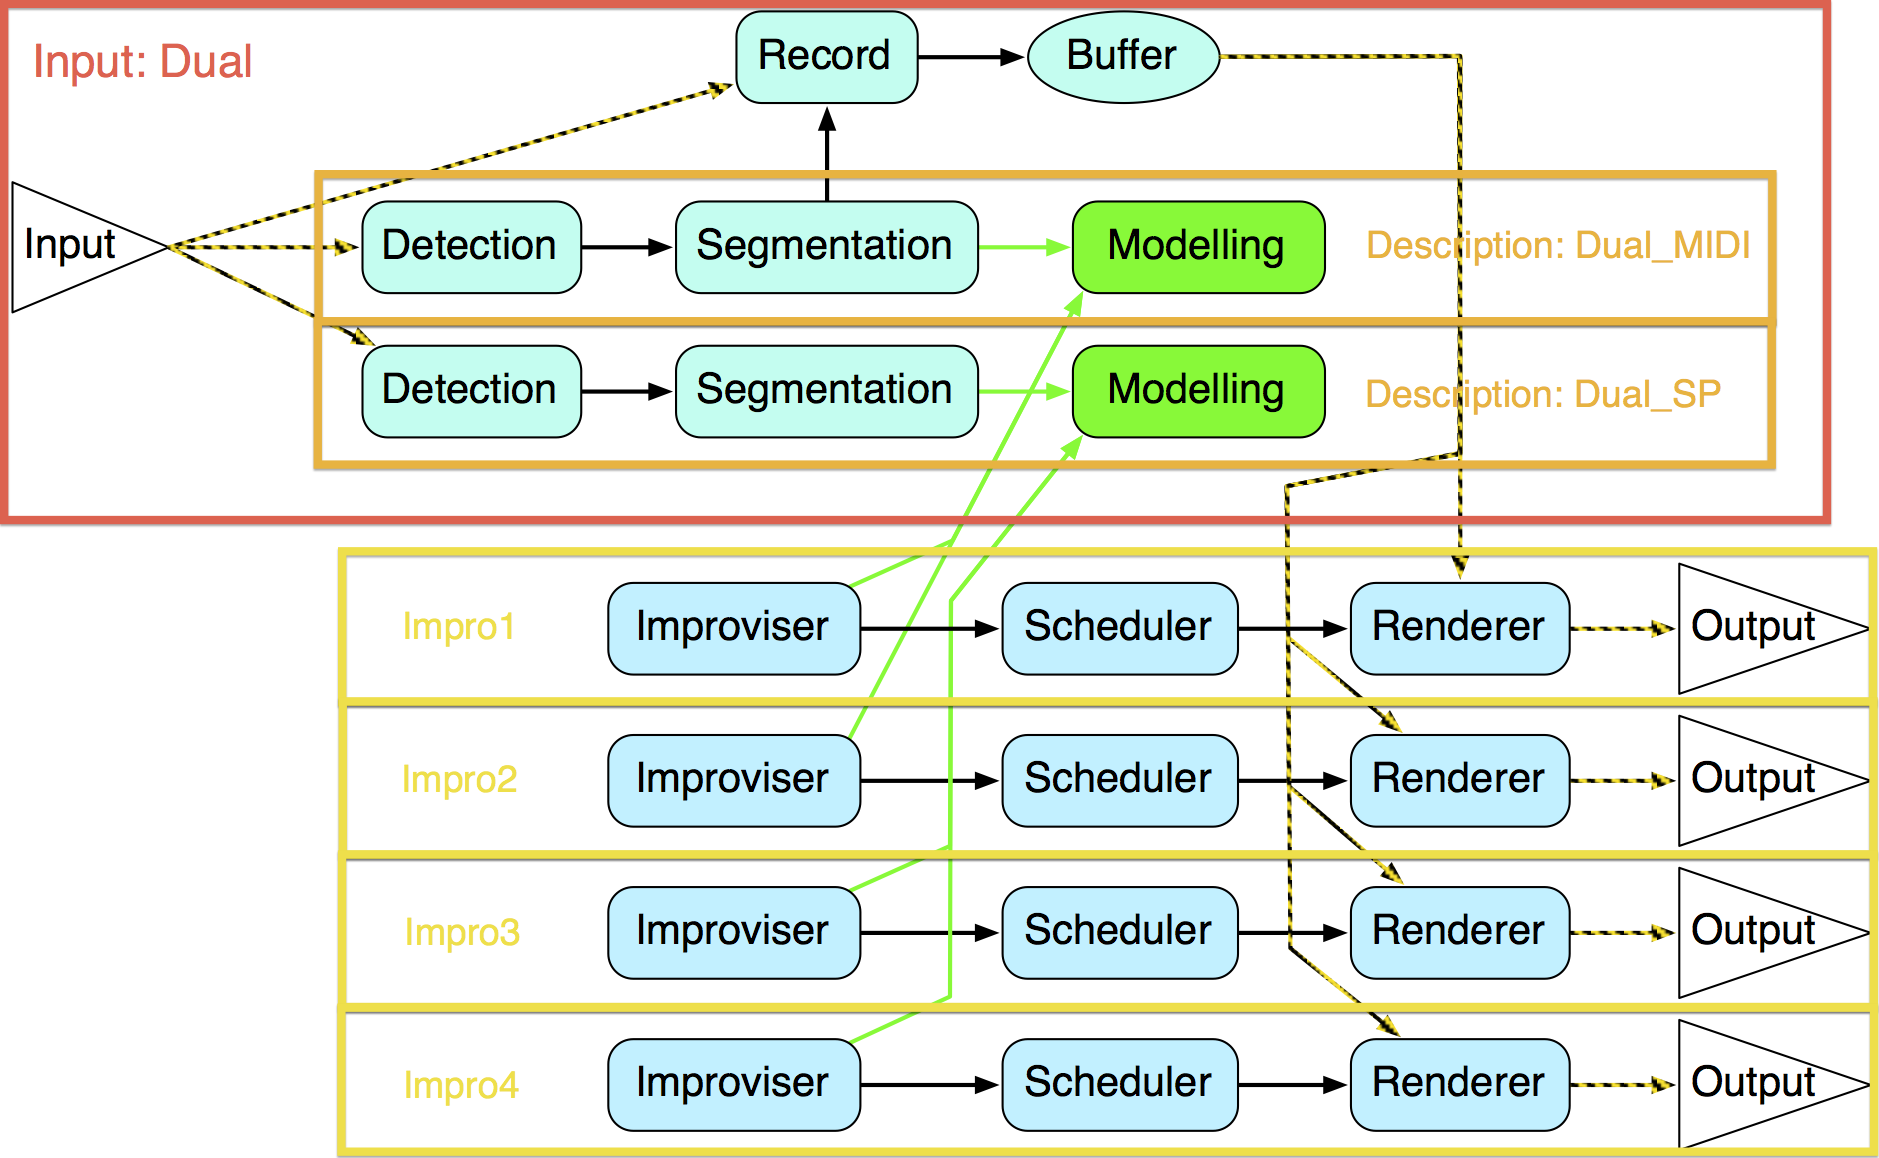
\includegraphics[width=0.75\linewidth]{Names.png}
	\caption{The differents names in OMax audio}
	\label{names}
\end{figure}
\par
There are 4 types of names: the first level is the name of the input. In the OMax 4.5.x patch, the audio input is named \textbf{Dual} and the MIDI input is named \textbf{MIDI}. Inside those input there can be different types of analysis/modeling chains which correspond to a second level of names. For example in the audio input of OMax 4.5.x, you can find two types of descriptions: pitch and spectral, the first description is referred as \textbf{Dual\_MIDI} (which is ambiguous and actually do not correspond to any MIDI processing but is an heritage of the previous versions of OMax). The spectral description of the \textbf{Dual} input is named \textbf{Dual\_SP}. The MIDI part of OMax 4.5.x (\textbf{MIDI} input) uses only one type of analysis and internal model named \textbf{MIDI\_POLY}.
\par
Each ``\,clone\,'' of OMax rely on an Improvisation core (see~\ref{core}). These cores are also named, so that the different players (see~\ref{players}) can effectively render the ``\,clones\,''. In the audio part of OMax 4.5.x, there are 4 improvisation cores named \textbf{Impro1}, \textbf{Impro2}, \textbf{Impro3} and \textbf{Impro4}. As explained on Figure~\ref{boxes}, the first two cores use the pitch description (\textbf{Dual\_MIDI}) while the last two cores use the spectral description of the input (\textbf{Dual\_SP}). The MIDI improvisation cores, \textbf{ImproM1} and \textbf{ImproM2} refer to the only available description of the MIDI input: \textbf{MIDI\_POLY}.
\par
Lastly, the visualization is also referred through its name. In the OMax 4.5.x patch, the visualization name is \textbf{Vizu} which correspond to the jitter window in which it is rendered. All the modules which have to draw in the visualization have to use this name. Figure~\ref{inspector} shows the usage of names for the module in charge of rendering the pitch description (\textbf{Dual\_MIDI}) in the visualization window (\textbf{Vizu}).
\subsection{Changing Names}
\begin{wrapfigure}[13]{R}{0.5\linewidth}
	\centering
	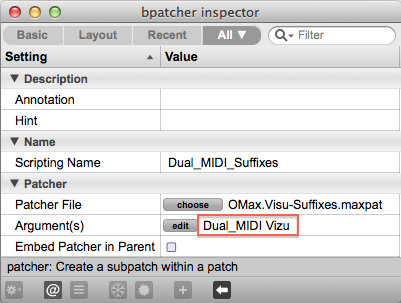
\includegraphics[width=0.9\linewidth]{Inspector.png}
	\caption[Name in a bpatcher Inspector]{}
	\label{inspector}
\end{wrapfigure}
All the names described in the previous section are mainly used as parameter of objects, abstractions or bpatchers. In the case of objects and abstractions, they are use explicitly as in Figure~\ref{boxes}. However, in the case of the bpatchers, those references are to be found in the bpatcher inspector (see Figure~\ref{inspector} for example). This makes the tracking of all the references in the OMax patch a very tedious task. However, if you would like for example to run two copies of the OMax patch, side by side in the same Max/MSP application, you will have to change every name of one of them.
\vspace*{2em} \\
Therefore an safer and faster method is given here:
\begin{itemize}
	\item Edit one of the copies of the patch in text mode (to benefit from search/replace functions). 
	\item Then do the following searches and replacements in this copy:\\
Caution! Doing search and replace, you need to keep extensions like \_MIDI, \_SP, \_POLY etc.
\indent	\begin{itemize}
		\item Search for all the mentions of ``\,Dual\,'' and replace them all by ``\,Duo\,'' (for example). This way, you will have independent audio inputs and models.
		\item Search for all the mentions of ``\,Vizu\,'' and replace them all by ``\,Disp\,'' (for example). This way, you will have 2 visualization windows.
		\item Search for all the mentions of ``\,Impro1\,'', ``\,Impro2\,'', ``\,Impro3\,'', ``\,Impro4\,'' and replace them by ``\,Clone1\,'', ``\,Clone2\,'', ``\,Clone3\,'', ``\,Clone4\,'' (for example).
	\end{itemize}
	\item If you are interested by the MIDI part of OMax as well:
\indent	\begin{itemize}
		\item Search for all the mention of ``\,$[$ "MIDI" $]$\,'' (brackets included with their content) and replace them all by ``\,$[$ "14H" $]$\,'' (for example)
		\item Search for all the mentions of ``\,MIDI\_POLY \,'' and replace them all by ``\,14H\_POLY\,'' (for example, or the same name you used for the previous step, appended with \_POLY).
		\item Search for all the mentions of ``\,ImproM1\,'' , ``\,ImproM2\,'' and replace them by ``\,ImproH1\,'' , ``\,ImproH2\,'' (for example)
	\end{itemize}
	\item Save the patch (with a different name than the ``\,original\,'' OMax patch)
	\item Finally load the ``\,orginal\,'' (not modified) OMax 4.5.x patch
	\item Then load the modified copy of the patch.
\end{itemize}
You should not have any error message when loading the second copy (either saying that a structure is missing or that the name is already in use) and everything should work well. Otherwise, you probably missed some name replacements.


%%%%%%%%%%%%%%%%%%%%%
%\chapter{Reference}
%\section{Patches Index}
%%
%\section{Parameter Index}
%%
%\section{Presets}

\nocite{*}
%\bibliographystyle{apalike}
%\bibliography{Doc.bib}

%\printbibliography
\printbibheading
\printbibliography[keyword=OMax,heading=subbibliography,title={OMax}]
\printbibliography[keyword=Improvisation,heading=subbibliography,title={Improvisation, Oracle}]
\printbibliography[keyword=Style Modeling,heading=subbibliography,title={Style Modeling}]
\printbibliography[keyword=Student works,heading=subbibliography,title={Student works}]

\end{document}